\chapter{Los misterios de Samotracia}

Los misterios de Samotracia, como indica el nombre, se dieron en la isla de Samotracia, estaban dedicados a los llamados\textit{ Theoi Megaloi} (Grandes Dioses) y estaban dedicados principalmente a dar seguridad en las empresas marítimas de los marineros griegos.

La historia pregriegra de Samotracia no goza tampoco de claridad; puede que los tirrenos hubieran intermediado en la isla si equiparamos el término kádmilos con el término latino camillus. También el término kásmilos puede tener su origen en los hititas. Si tomamos como mitología, la de la salvación de Dárdano -la cual me resulta más convincente- tendríamos analogías con algunos misterios de Méter en Asia Menor, igual que los misterios eleusinos.

Lo que sí se conoce, es que los misterios samotracios estaban bastante extendidos en Grecia en el siglo V a. C. según Guettel\footcite[4-5]{guettelcoleTheoiMegaloiCult1984}; Burkert afirma que la actividad religiosa comenzó en el siglo VII a. C.\footcite[376]{burkertReligionGriegaArcaica2007}.

Los dioses de Samotracia tuvieron relevancia en todo el mediterráneo, habiéndose llevado a cabo hasta la época de Constantino\footcite[376]{burkertReligionGriegaArcaica2007}. El período helenístico fue el mejor para los misterios de Samotracia. Reflejo de ello es la gran cantidad de inscripciones que mencionan los \textit{theoi} de Samotracia en lugares fuera de la isla\footcite[21]{guettelcoleTheoiMegaloiCult1984}. El culto tuvo iniciados griegos y romanos; aunque fueron los griegos quienes establecieron sacerdocios, festivales y santuarios dedicados a los dioses de Samotracia en sus ciudades, a diferencia de los romanos, que aunque haya constancia de que visitaron Samotracia, no existen vestigios en Roma de dedicaciones de ningún tipo a los \textit{theoi Megaloi}\footcite[5]{guettelcoleTheoiMegaloiCult1984}.
 
La ubicación fue un punto clave en el desarrollo del culto: una isla accesible desde Tracia y Asia Menor, rocosa y montañosa. Por ello no extraña que las divinidades asociadas a la isla tuvieran poderes sobre el mar. 

\section{Origen y mitología}

La mitología de Samotracia ha sido un tema ampliamente discutido. Diferentes autores han aportado varias interpretaciones sobre cuál es el mito en el que se basa este culto. El desconocimiento surge de que, hasta ahora, se han mantenido en secreto  el nombre de los dioses a los que se rendía culto en la isla. Tradicionalmente se habían identificado los dioses con \textit{Kabeiroi}, deidades a las que se rendía culto en Lemnos y Tebas. 
Burkert los identifica, a partir de la lectura de Varron, con Júpiter, Juno y Minerva\footcite[377]{burkertReligionGriegaArcaica2007}; pero Guettel lo refuta ya que el autor clásico, sin haber conocido los misterios de la isla, buscaba era enaltecer la figura de la triada capitolina como \textit{dei magni} de Roma\footcite[2-3]{guettelcoleTheoiMegaloiCult1984}.

Fue Herodoto quien identificó a los \textit{Theoi Megaloi} de Samotracia con los cabiros; pero la idea se refutó\footcite[377]{burkertReligionGriegaArcaica2007} porque el término Kabeiroi no aparecía en ninguna de las inscripciones en el recinto de culto de Samotracia, además que los cabiros estaban dedicados al trabajo del metal y en Samotracia la iniciación ofrecía en un principio protección en el mar\footcite[2-3]{guettelcoleTheoiMegaloiCult1984}.

\textit{"Y cualquiera que esté iniciado en los misterios de los Cabiros (que celebran los samotracios por haberlos heredado de los pelasgos), ese iniciado sabe lo que estoy diciendo; pues esos pelasgos que pasaron a convivir con los atenienses habitaban, antaño, Samotracia y, de ellos, heredaron los samotracios los misterios"}\footcite[341]{herodotoHistoriaLibroII1992}.

Otra línea interpretativa defiende la identificación de una Gran Diosa de Samotracia con Méter, ya que en monedas de la isla aparecía la diosa Cibeles. Acompañando a esta diosa tendríamos a un dios servidor llamado Kádmilos, que se ha traducido como Hermes. Podría estar relacionado, ya que en ñas celebraciones de los misterios en Samotracia se sacrificaba un carnero\footcite[378]{burkertReligionGriegaArcaica2007}.

También podría haberse venerado a un joven dios-servidor llamado Kásmilos o Kádmilos, en relación con Cadmo, quien había celebrado su boda en Samotracia.

Burkert también nos muestra otra visión en la que los misterios estarían relacionados con la mitología heroica samotracia existente. Electra, señora de Samotracia, 'la radiante', tiene tres hijos con Zeus: Dárdano, Eetión o Yasión y Harmonia. Esta última se casa con Cadmo de Tebas, pudiendo haber aquí también una relación entre Cadmo y Kádmilos. Dárdano debe huir de la isla al asesinar a su hermano Yasión, y lo hace en una balsa mientras mientras ocurre un gran diluvio. Acaba desembarcando en el monte Ida, donde instaura la estirpe de los troyanos e introduce el culto de Méter Idaíe\footcite[378]{burkertReligionGriegaArcaica2007}.

Esta interpretación adquiere sentido al tener puntos de conexión con el culto mistérico, porque el hecho de que un criminal sea salvado en las aguas recuerda a la pregunta que se realiza en la ceremonia mistérica sobre qué es lo peor que han realizado los iniciados en sus vidas, y también recuerda a la salvación de Odiseo gracias al velo y a la balsa\footcite[378]{burkertReligionGriegaArcaica2007}.

Hugh Bowden, en \textit{Ancient Mystery Cults}\footcite[80-81]{bowdenMysteryCultsAncient2023}, busca una explicación para la falta de información sobre los dioses de la isla. Identifica tres posibles teorías que mostramos a continuación. 

La base mitológica de los griegos fue Homero y Hesíodo, quienes crearon y ordenaron toda una genealogía de olímpicos dotándolos de un relato. A partir de la obra de estos autores se desarrolló también la base artística y poética de las divinidades. Pero en muchas ciudades griegas se veneraba a distintas deidades que no aparecían en estos poemas. Y además, no tenían porque ser ni dioses individuales, y esto lo podemos observar en la acepción de los \textit{theoi megaloi}  de Samotracia y en los cabiros de Lemnos y Tebas. La información de la identidad de los dioses podría ser el secreto, o parte de este. No es el caso de Eleusis, donde este contenido no parecía ser el secreto. 

Otra visión interesante es que los griegos también encontraban dioses en los lugares que habitaban, no a partir de la literatura existente. Esto significaba que las personas de Samotracia no tenían porqué conocer al completo a las deidades, y eso dificultaba la identificación de la deidad por parte de los devotos. Esta no identificación generaba la existencia de dioses sin un relato a su alrededor: dioses sin mito.

Por último, Bowden explica la existencia de una identificación 'no excluyente'. Nos muestra lo que ocurría en Delos; el sacerdote era nombrado 'Sacerdote de los Grandes Dioses de Samotracia, los Dioscuros, los Cabiros'. El autor interpreta esta mención como un 'no compromiso' por parte de la población de Delos a identificar los dioses adorados allí. 

El autor concluye que los \textit{Theoi Megaloi} de Samotracia no son dioses homéricos, como ocurre con los Cabiros. Puede que ese hecho hiciera que compartieran características y por eso Heródoto llegó a  identificar los dioses de Samotracia con los Cabiros\footcite[82]{bowdenMysteryCultsAncient2023}. 

\section{Desarrollo del culto: Participación y Acceso}\sectionmark{Desarrollo del culto}

En los muros de la estoa se descubrió una lista de nombres que parece indicar las personas que se habían iniciado en los misterios, y que provenían de difrentes lugares del Egeo y Mediterráneo. Gracias a esas inscripciones se conoce más ampliamente el desarrollo de los misterios.

La ceremonia para conseguir el estatus de \textit{mystai} se realizaba en el \textit{anaktoron}.
En la cámara norte del \textit{anaktoron} se encontraba una inscripción que limitaba el paso a las personas que no hubiesen alcanzado la \textit{myesis}. Por eso, se cree que el rito de iniciación se celebraba en la sala central previa a la cámara norte. 
En la entrada del edificio se encontraba una estructura circular, llamada \textit{bothros}, que rodeaba un pozo de cinco metros de profundidad. Susan Guettel las identifica como estructuras destinadas a realizar libaciones. 
En el extremo sur del \textit{anaktoron} encontramos otra sala que no estaba conectada a la sala principal de iniciaciones, seguramente porque era el lugar donde los participantes se cambiaban de vestimenta para acceder por el exterior al extremo oeste del edificio. 

Los bancos del interior de la habitación principal habrían sido utilizados para observar las ceremonias allí dentro celebradas. Dentro de la sala han sido encontrados objetos de bronce, cerámica sencilla, cuchillos de hierro y un gran escudo de bronce. Guettel sugiere que ese escudo estaba dedicado a realizar una danza al estilo de los coribantes, quienes saltaban y golpeaban escudos \footcite[29]{guettelcoleTheoiMegaloiCult1984}.

Lo que se realizaba dentro del edificio seguramente estuviera relacionado con la revelación de ciertos objetos sagrados, seguramente almacenados en la cámara norte con acceso restringido que hemos mencionado anteriormente. 

Posteriormente, los iniciados se desvestían y lavaban para colocarse una faja púrpura en torno al abdomen, lo que podría estar relacionado con el momento en que Odiseo tiró sus ropas a la tempestad para zambullirse con el velo de Leucótea\footcite[377]{burkertReligionGriegaArcaica2007}. Después, a cada iniciado se le entregaba un anillo de hierro -a veces con una pieza de oro en él- que portarían el resto de su vida. Se han encontrado anillos de este tipo en el santuario y en una tumba samotracia \footcite[30]{guettelcoleTheoiMegaloiCult1984}. Una vez son \textit{mystai} acceden a la sala norte del edificio para que se les revelasen los secretos o se les mostrasen ciertos objetos.

La ceremonia continuaría en el \textit{hieron}, donde solo acceden los \textit{mystai} para poder realizar la \textit{epopteia}. Se conoce que el \textit{hieron} estaba destinado a esta segunda etapa iniciática por la inscripción de la entrada, que prohibía el acceso a quien no hubiera realizado la \textit{myesis} \footcite[302]{burkertReligionGriegaArcaica2007}.

En los escalones fuera del edificio el sacerdote preguntaría a los mystai qué es lo peor que han realizado en su vida. Guettel desecha la idea de que la intención sea realizar un juicio moral, sino que busca conocer la pureza del iniciado para no contaminar el santuario \footcite[32]{guettelcoleTheoiMegaloiCult1984}. Burkert, en cambio, defiende la idea de que esta cuestión que realiza el sacerdote a los iniciados está dedicada a estrechar el vínculo entre los asistentes \footcite[376]{burkertReligionGriegaArcaica2007}. En esos mismos escalones Guettel cree que los iniciados realizaban el juramento de silencio, por el que no podían desvelar los secretos que se revelaban en el interior \footcite[32]{guettelcoleTheoiMegaloiCult1984}.

Luego de este proceso en la entrada del \textit{hieron}, los \textit{mystai} se colocaban en el pórtico mientras esperaban a poder acceder al interior. A la derecha de la puerta se encontraba un desagüe de gran capacidad, cuya función -se cree- era llevarse el agua de una especie de purificación que se llevaba a cabo con agua.

Una vez dentro del hieron, los presentes ocupaban los bancos de la habitación principal. Dentro del edificio se encontraba la \textit{eschara}, un altar circular que ocupaba un lugar central dentro de la sala. Eso hace suponer que era el lugar para realizar algún rito previo a la \textit{epopteia}, ya que además se encontraron huesos de aves en su interior.

Ahora nos trasladaremos al ábside del \textit{hieron}, donde seguramente se celebraba la \textit{epopteia}. El ábside disponía en su interior una plataforma de mármol (\textit{bema}), que sería ocupada por el sacerdote que oficiaba la ceremonía. Lo que se realizaba en el momento de la \textit{epopteia} no se puede concretar.

Hemos mencionado previamente las inscripciones de listas de iniciados que se encontraron en Samotracia (dentro y fuera del santuario). Ahora desgranaremos la información que han aportado sobre las personas asistentes a los misterios. 

Estas listas cuentan con más de cien inscripciones sobre los iniciados en los misterios, y además diferenciaban si la persona era mystai o epoptai. También podían indicar la polis de origen de la persona en cuestión, quien podía ser, en su mayoría un ciudadano común o un esclavo. Las iniciaciones en los misterios de Samotracia podían realizarse en cualquier momento del año, aunque muchas se llevaban a cabo en junio, mes en el que era más seguro llevar a cabo expediciones marítimas. Y en relación con este hecho, se descubrió que tres de las listas de \textit{epoptai} estaban fechadas en junio, quizás -indica Guettel- porque la segunda fase de iniciación solo se celebraba en este mes.
A partir de estas listas, también conocemos que las iniciaciones solían realizarse en grupos de \textit{theoroi} (embajadores religiosos), de familiares o de personas pertenecientes al mismo barco. Aunque los misterios fuesen accesibles a todo el público, se ha observado que el número de mujeres asistentes es muy reducido, debido a que la isla es más accesible para los marineros \footcite[38-44]{guettelcoleTheoiMegaloiCult1984}.

Los misterios samotracios eran ampliamente conocidos en Grecia; son treinta y cuatro las ciudades que mencionan \textit{Theoi Megaloi} \footcite[88]{moralgarciaInfluenciaMisteriosSamotracia2020}, y en las \textit{Argonaúticas} de Apolonio de Rodas, los navegantes realizan una parada en Samotracia para iniciarse en los misterios y ganar seguridad en el trayecto marítimo.
\textit{
"Al atardecer, por instrucciones de Orfeo, atracaron en la isla de la Atlántida Electra, para conocer, mediante piadosas iniciaciones, los ritos secretos y así navegar seguros sobre el espantoso mar. Acerca de éstos ya no extenderé más mi relato, sino que salud a la propia isla así como a sus divinidades locales, quienes patrocinan aquellos misterios que no es lícito cantar"} \footcite[132]{derodasArgonauticas1996}.





\section{El santuario}

La construcción del santuario de Samotracia data del siglo IV a. C., aunque se conoce que los misterios samotracios ya estaban bastante extendidos en Grecia en el siglo V a. C. según Guettel; Burkert afirma que la actividad religiosa comenzó en el siglo VII a. C.. El santuario se encuentra en un valle de las afueras de la ciudad, entre dos colinas, una situada al este y otra hacia el oeste. 

Se llegaba al lugar por un sendero que comenzaba en el norte, en la ciudad. Se entraba por los propileos e inmediatamente aparecía un  pequeño edificio dórico en la colina oeste. Desde allí se llegaba a la zona principal del santuario.

\begin{figure}[h!]
	\centering
	\begin{subfigure}[t]{0.45\linewidth}
		\centering
		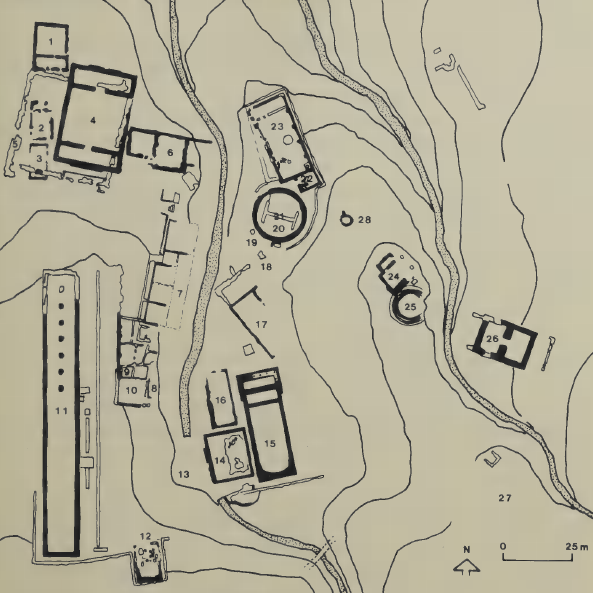
\includegraphics[width=\linewidth]{Imagenes/PlanoSantuarioDeSamotracia}
		\caption{\textit{Plano del Santuario}\footcite[8]{guettelcoleTheoiMegaloiCult1984}.}
		\label{fig:santuario-samotracia}
	\end{subfigure}
	\begin{subfigure}[t]{0.45\linewidth}
		\centering
		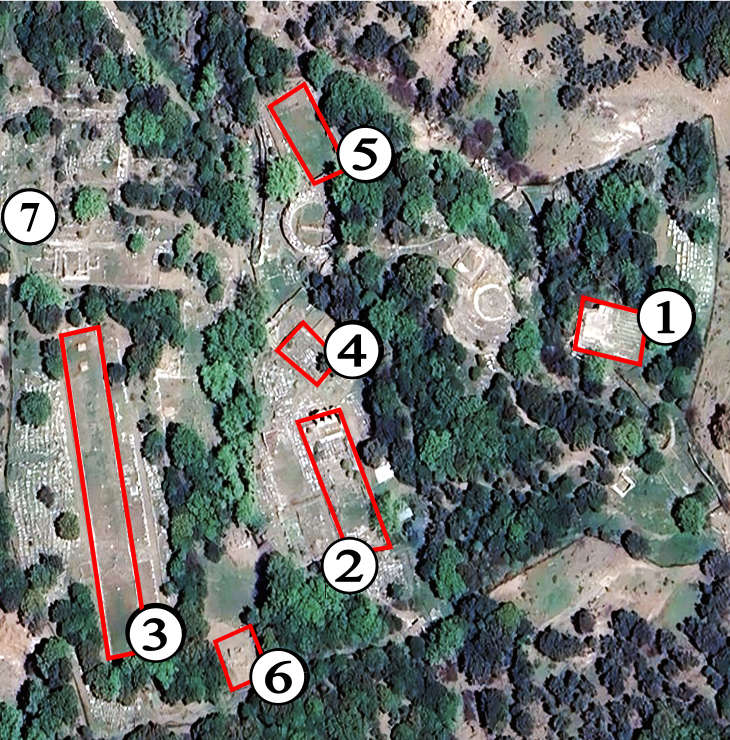
\includegraphics[width=\linewidth]{Imagenes/VistaAereaSamotracia}
		\caption{\textit{Vista Aérea. 1: Propileos; 2: Hieron; 3: Estoa; 4: Temenos; 5: Anaktoron; 6: Fuente de Niké; 7: Edificios del tesoro. Google Earth.}}
		\label{fig:vista espacial-samotracia}
	\end{subfigure}
	\caption{\textit{Santuario de Samotracia}}
	\label{fig:westminster}
\end{figure}

Los edificios más relevantes son los llamados \textit{hieron} y \textit{anaktoron}, ya que eran los lugares donde se realizaban los procesos de iniciación. Al segundo se llegaba siguiendo la orilla oriental del arroyo -antiguamente dos arroyos corrían por el valle- hacia el norte. El \textit{anaktoron} era un edificio de forma rectangular dividido en tres espacios, entre los cuales, el central serviría para llevar a cabo la \textit{myesis }, etapa de iniciación de los devotos para convertirse en \textit{mystai}, ya que estaba equipado con una bancada.

El \textit{hieron} se encontraba hacia el sur del \textit{anaktoron}; era el mayor de tres edificios, y en él se celebraría la \textit{epopteia}, fase de contemplación, y en el que los devotos adquirirían la clase de \textit{epoptai}. Estas dos fases principales en las celebraciones mistéricas también ocurren en los misterios eleusinos.

Al norte del hieron encontramos también un edificio, denominado temenos, cuyo recinto principal es una zona sin techo en la que se encontraban un \textit{bothros} (pozo) y una \textit{eschara} (altar-hogar), que servían, según Guettel para celebrar ceremonias de preparación para la iniciación.

Cabe destacar el edificio situado en la zona más occidental. Se trata de la estoa, de forma rectangular y alargada, que servía de refugio para los visitantes de Samotracia. En sus muros se encontraban las listas de los visitantes e iniciados que visitaron en el santuario. Al norte de este edificio se han identificado dos pequeños edificios contiguos que podrían haber servido para custodiar el tesoro. Por último, encontramos cerca de la estoa, hacia el sureste, la Fuente de Niké, donde habría estado colocada la famosa estatua de Niké \footcite[8]{guettelcoleTheoiMegaloiCult1984}. 

Hemos mostrado las estructuras del santuario que están relacionadas con los misterios de Samotracia. Existen numerosas estructuras más en el lugar, pero no se ha encontrado una función clara para todas ellas; es por ello que nos centraremos en las mostradas aquí.
 

\section{Símbolos e iconografía} 

Si bien el culto a los \textit{Theoi Megaloi} no goza de una basta iconografía, en su santuario se encontraba la famosa Niké de Samotracia, gran escultura helenística atribuida al escultor Pitócrito. Me resulta interesante explicar la historia de esta escultura para poder dimensionar mejor el papel de este culto mistérico en el pensamiento griego.

\begin{figure}[h!]
	\centering
	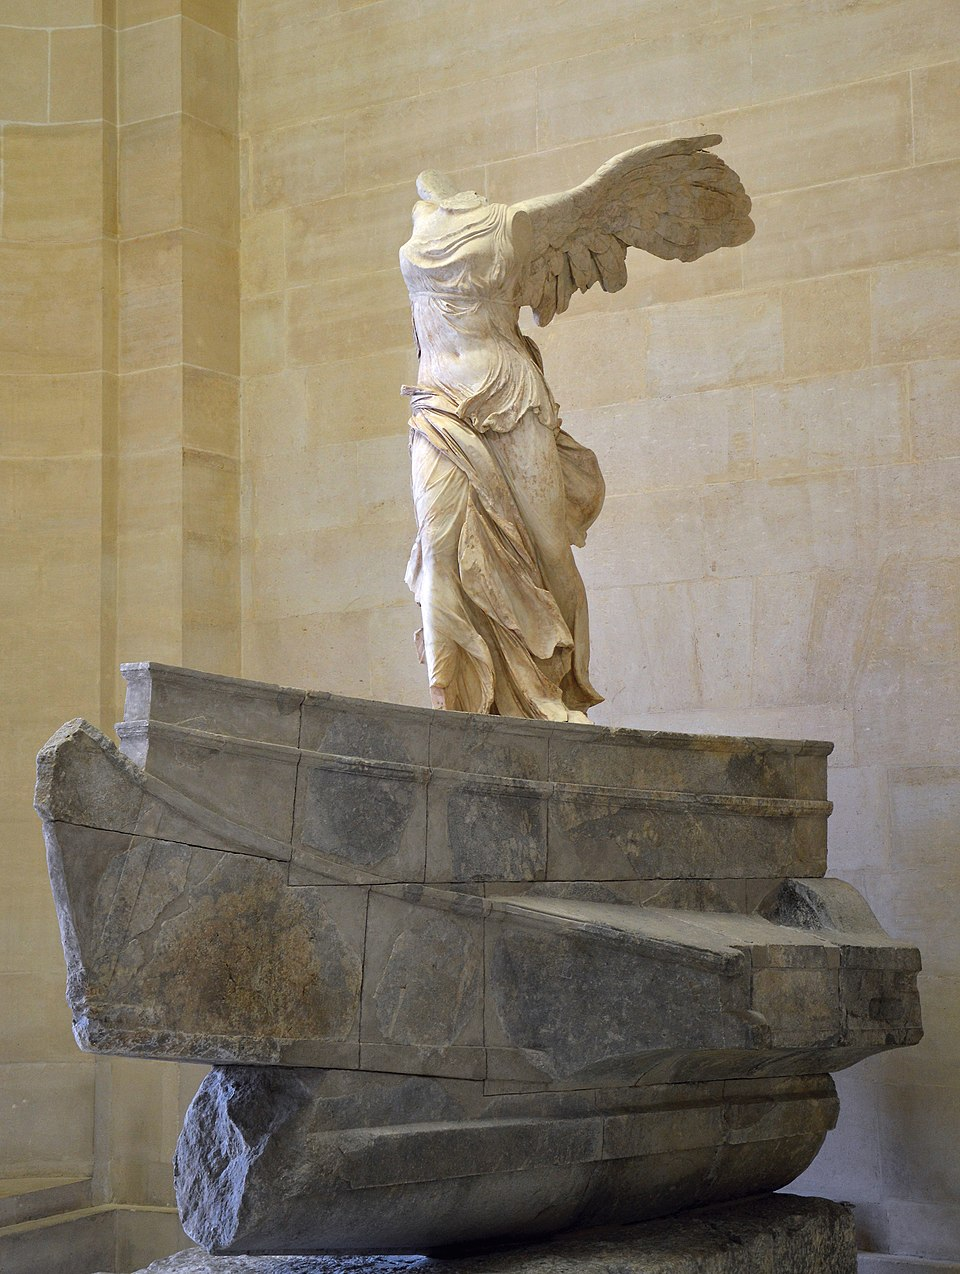
\includegraphics[width=0.45\linewidth]{Imagenes/VictoriaSamotracia}
	\caption{\textit{Niké de Samotracia (s. II a. C.), Museo del Louvre}.}
	\label{fig:nike-samotracia}
\end{figure}

La escultura es una ofrenda dedicada a los Grandes Dioses de Samotracia, cuya función estaba fuertemente ligada con las empresas marítimas. Por el dinamismo de sus ropajes, Niké esta guiando el barco mientras lucha con una gran tempestad marítima. La estatua está tallada en mármol blanco de Paros, mientras que la base está hecha en piedra larcia azul grisácea importada de Rodas. Esta base, tenía un peso de 30 toneladas, más el peso de 5 toneladas de la escultura de Niké. Esto constituía un gran cargamento para un comerciante griego mediano\footcite[403]{stewartNikeSamothraceAnother2016}. 

La participación de Rodas en la dedicación es presente, por el uso de la piedra larcia y porque en las inscripciones de la estoa del santuario los rodios aparecen en gran medida como embajadores sagrados e iniciados. Además, las dedicaciones para los \textit{Theoi Megaloi} en Rodas son muy abundantes.

Andrew Stewart busca una explicación para saber el motivo por el que Rodas (ciudad a quinientos kilómetros de distancia de Samotracia) dedicó esta gran estatua. 

Rodas libró varias batallas durante el siglo II a. C. y obtuvieron, con bastante seguridad, siete victorias marítimas. EL origen de la ofrenda está en las guerras ocurridas entre Prousias II Kynegos y Átalo II Filadelfio de Pérgamo. 

\begin{figure}[h!]
	\centering
	\includegraphics[width=0.45\linewidth]{Imagenes/ReconstrucciónFuente}
	\caption{\textit{Fuente de Niké en el santuario. Reconstrucción hipotética realizada por Bonna Wescoat y Chase Jordan \footcite[401]{stewartNikeSamothraceAnother2016}.}}
	\label{fig:fuente-nike}
\end{figure}

En una primera contienda, Prousias salió victorioso en el ataque al Nicéforo y saqueó los templos y santuarios, llevándose consigo las imágenes sagradas de los dioses. Después de esta conducta hacia los dioses sufre, en la Propóntide una tormenta que causó el hundimiento de la mayor parte de sus navíos \footcite[404]{stewartNikeSamothraceAnother2016}.

Átalo, después de la derrota planeó durante un año la ofensiva hacia Prousias. Se dedicó a movilizar a sus aliados, entre los que figuraban los rodios. El ataque estaba destinado a Birtinia. Átila y los aliados hostigaron gravemente a las ciudades bajo dominación de Prousias.

Stewart concluye que la Niké es rodia o pérgamo-rodia, ya que los \textit{Theoi Megaloi }actuaron a favor de ellos en la gran batalla contra Prousias\footcite[405]{stewartNikeSamothraceAnother2016}. El hecho de que la isla de Rodas dedicara esta gran estatua a una isla a quinientos kilómetros de distancia demuestra la importancia que tenían los misterios de Samotracia para los navegantes.


\section{Función y significado}

La iniciación en Samotracia otorgaba protección en el mar, en batalla y finalmente, después de la muerte\footcite[6]{guettelcoleTheoiMegaloiCult1984}. Aunque Bowden niega que tengan alguna relación con la escatología \footcite[82]{bowdenMysteryCultsAncient2023}.

Susan Guettel propone una teoría a partir de las estatuas itifálicas que se encontraban en la entrada de los edificios principales de la iniciación: estaban relacionados con la actividad sexual y el origen de la vida \footcite[29]{guettelcoleTheoiMegaloiCult1984}, pero parece que esta hipótesis no ha tenido más recorrido. 

Los autores como Susan Guettel y Hugh Bowden indican la protección marítima que ofrecían los misterios. El artículo de Carlos Moral en el que presenta una hipótesis para la funcionalidad de los misterios samotracios \footcite[]{moralgarciaInfluenciaMisteriosSamotracia2020} profundiza en la relación de Samotracia con la vida marítima y establece que los misterios de Samotracia funcionaban a nivel religioso, mitológico, político y económico. 

Moral indica que los costes de las iniciaciones serian bastante elevados ( y aumentarían según el nivel de iniciación), puede ser esta la razón por la que de las cien inscripciones, sólo dieciocho son de \textit{epoptai}. El control de las vías marítimas conferían a su vez poder económico y político, y el poder marítimo estaría condicionado por el poder económico. Entonces el autor establece que los misterios podían funcionar como una especie de garante de poder. los viajes a la que los marineros debían dedicar una partida de los presupuestos expedicionarios para cubrir las ofrendas de iniciación y contar con la protección divina de los Grandes Dioses \footcite[93]{moralgarciaInfluenciaMisteriosSamotracia2020}.

Por otro lado, el santuario también funcionaría como un punto de encuentro para los marineros en los que intercambiar información sobre nuevas rutas comerciales, rumores e intereses comerciales \footcite[95]{moralgarciaInfluenciaMisteriosSamotracia2020}. Esta información resultaba de gran relevancia ya que los \textit{emporos} (comerciantes a gran escala) griegos debian viajar constantemente y tomar iniciativas sobre la marcha del viaje\footcite[254]{villalbababiloniComerciantesGranEscala2022}.

Otro punto relevante que desarrolla Moral es la asistencia de los \textit{theoroi} (embajadores religiosos), lo que indica el interés público en los misterios y que estos funcionaran como un seguro comunitario de viaje. Además, compartirían información sobre los puertos de las polis entre los demás emisarios. 

Tampoco hay que obviar el respeto que los griegos tenían al mar, sobre todo a morir en él. El mar era un espacio desconocido y existían historias de monstruos y espíritus marinos. Además, morir en el mar significaba no tener posibilidad de un enterramiento, por lo que el alma del difunto vagaría por toda la eternidad \footcite[93]{fernandeznietoMorirAguaMorir2012}.  

Esta teoría de Carlos Moral no significa que hubiera personas que se iniciaran en los misterios por protección marítima. Si bien es cierto que la mayoría de asistentes eran marineros y tampoco es inusual que los santuarios en la Antigua Grecia sirvieran como punto de reunión, quizás su desarrollo hizo que el culto se convirtiera en un papel fundamental de las prácticas comerciales.
